% VLDB template version of 2020-08-03 enhances the ACM template, version 1.7.0:
% https://www.acm.org/publications/proceedings-template
% The ACM Latex guide provides further information about the ACM template




\documentclass[sigconf, nonacm]{acmart}
\usepackage{soul}


\usepackage[demo]{graphicx}
\usepackage{subcaption}

%% The following content must be adapted for the final version
% paper-specific
\newcommand\vldbdoi{XX.XX/XXX.XX}
\newcommand\vldbpages{XXX-XXX}
% issue-specific
\newcommand\vldbvolume{14}
\newcommand\vldbissue{1}
\newcommand\vldbyear{2020}
% should be fine as it is
\newcommand\vldbauthors{\authors}
\newcommand\vldbtitle{\shorttitle} 
% leave empty if no availability url should be set
\newcommand\vldbavailabilityurl{URL_TO_YOUR_ARTIFACTS}
% whether page numbers should be shown or not, use 'plain' for review versions, 'empty' for camera ready
\newcommand\vldbpagestyle{plain} 


\begin{document}
\title{Semantic Segmentation on Satellite Imagery (must change*)\\}

\author{Nancy Nigam}
\affiliation{%
  \institution{New York University}
}
\email{nn2163@nyu.edu}

\author{Jorge Roldan}
\affiliation{%
  \institution{New York University}
}
\email{jlr9718@nyu.edu}

\author{Aditya Upadhyaya}
\affiliation{%
  \institution{New York University}
}
\email{au2056@nyu.edu}


\maketitle


\begin{abstract}
\hl{Do abstract when we are done with everything else}
\end{abstract}

% ============================
\section{Introduction}
% ============================

% ============================
\section{Related Work}
% ============================
Start talking about \cite{DBLP:journals/corr/abs-2003-02899}. \\ \indent


Talk about this \cite{DBLP:journals/corr/abs-2010-06285}. \\ \indent



Continue talking about this paper \cite{DBLP:journals/corr/abs-1911-12903},




% ============================
\section{Datasets}
% ============================
% ----------------------------------------
\subsection{LandCoverNet Dataset}
% ----------------------------------------
\begin{table}[htbp]
\centering
\caption{LandCoverNet dataset}
\begin{tabular}{|p{1.8cm}|p{0.6cm}|p{1.6cm}|}
 \hline
 \multicolumn{3}{|c|}{\textbf{LandCoverNet Dataset Classes}} \\
 \hline
 \textbf{Class Name} & \textbf{Pixel Value}& \textbf{RGB Value} \\
 \hline
 Unkown & 0  & (0,0,0)\\ 
 \hline
 Water & 1  & (0,0,255)\\ 
 \hline
 Artificial & 2  & (136,136,136)\\ 
 \hline
 Natural & 3  & (209,164,109)\\ 
 \hline
 Snow/ice & 4 &  (245,245,255)\\ 
 \hline
 Wooddy & 5  & (214,76,43)\\ 
 \hline
 Cultivated & 7  & (24, 104, 24)\\ 
 \hline
 (Semi) Natural & 7  & (0, 255, 0)\\ 
 \hline
\end{tabular}
\label{landcovernet_dataset}
\end{table}

\subsection{Semantic Segmentation of Crop Type in Ghana Dataset}
\subsubsection{Dataset Characteristics}


\begin{table}[htbp]
\centering
\caption{Ghana Dataset}
\begin{tabular}{|p{2.2cm}|p{0.7cm}|p{1.6cm}|}
 \hline
 \multicolumn{3}{|c|}{\textbf{Crop Type in Ghana Dataset Classes}} \\
 \hline
 \textbf{Class Name} & \textbf{Pixel Value}& \textbf{RGB Value} \\
 \hline
  Unknown & 0  &  (0, 0, 0)\\ 
 \hline
  Ground nut & 1  & (80,0,165) \\ 
 \hline
  Maize & 2  & (255,204,0) \\ 
 \hline
  Rice & 3  & (0,244,244)\\ 
 \hline
  Soya bean & 4  & (105,105,105)\\ 
 \hline
  Yam & 5  & (255,255,102) \\ 
 \hline
  Intercrop & 6  & (255,153,153)\\ 
 \hline
  Sorghum & 7  & (127,222,209)\\ 
 \hline
  Okra & 8  & (222,127,219)\\ 
 \hline
  Cassava & 9  & (108,67,107)\\ 
 \hline
  Millet & 10  & (152,134,94)\\ 
 \hline
  Tomato & 11 & (99,228,150) \\ 
 \hline
  Cowpea & 12  & (99,176,228)\\ 
 \hline
  Sweet Potato & 13 & (255,186,186)\\ 
 \hline
  Babala Beans & 14  & (204,0,102) \\ 
 \hline
  Salad Vegetables & 15  & (102,51,0)\\ 
 \hline
  Bra and Ayolo  & 16  & (204,204,255)\\ 
 \hline
  Watermelon & 17  & (0,102,204)\\ 
 \hline
  Zabla & 18 & (255,0,255)\\ 
 \hline
  Nili & 19 & (102,0,204)\\ 
 \hline
  Kpalika & 20 & (141,51,117)\\ 
 \hline
  Cotton & 21 & (145,187,192)\\ 
 \hline
  Akata & 22 & (155,123,219)\\ 
 \hline
  Nyenabe & 23 & (193,0,76)\\ 
 \hline
  Pepper & 24 & (204,255,153)\\ 
 \hline
\end{tabular}
\label{ghana_dataset_class_table}
\end{table}

\subsection{LandCover.ai Dataset}



\subsubsection{Dataset Characteristics}
The LandCover.ai dataset consists of satellite imagery for semantic segmentation applications covering a region of Poland of a total area of 216.2 km$^2$ \cite{DBLP:journals/corr/abs-2005-02264}. The original dataset consists of 41 orthophoto tiles of 5 km$^2$ where 33 images and 8 images have a resolution of (9000 px x 9500 px) and (4200 px x 4700 px), respectively. \\ \indent
The authors of this dataset \cite{DBLP:journals/corr/abs-2005-02264} provided a script which we used to split these 41 images and their respective masks into 10,674 source and 10,674 masks images of (512 px x 512 px) resolution. These land cover of these images consist of agricultural areas (60 \%) and mixed forests (29.6 \%). \\ \indent



\subsubsection{Classes and RGB Mapping}
The name of the classes, their respective pixel value and RGB value are shown in table \ref{landcover_ai_classes}. The annotations were made manually by the authors using VGG  Image Annotator (VIA) \cite{dutta2019vgg}. According to \cite{DBLP:journals/corr/abs-2005-02264}, there are 12280 buildings (1.85 km$^2$), 72.02 km$^2$ of woodland, 13.15 km$^2$ of water, 3.5 km$^2$ of raods, and 125.75 km$^2$ of background, that is, the unknown class.

\begin{table}[htbp]
\centering
\caption{LandCover.ai Dataset}
\begin{tabular}{|p{1.2cm}|p{0.7cm}|p{1.6cm}|}
 \hline
 \multicolumn{3}{|c|}{\textbf{Landcover.ai Dataset Classes}} \\
 \hline
 \textbf{Class Name} & \textbf{Pixel Value}& \textbf{RGB Value} \\
 \hline
 Unknown & 0  & (0,0,0)\\ 
 \hline
 Building & 1  & (80,0,165)\\ 
 \hline
 Woodland & 2  & (255,204,0)\\ 
 \hline
 Water & 3  & (0,244,244)\\ 
 \hline
 Road & 4  & (105,105,105)\\ 
 \hline
\end{tabular}
\label{landcover_ai_classes}
\end{table}

\subsubsection{Data preprocessing}


% ============================
\section{Methodology}
% ============================
% ----------------------------------------
\subsection{Architectures}

For the purpose of our experiments, we leverage a U-Net network \cite{ronneberger2015unet}. U-Net is a fully convolution neural network used extensively for image segmentation. It involves encoder and decoder components connected with skip connections. For the classification model that serves as our encoder and extracts features of different spatial resolution, we use a ResNet architecture \cite{DBLP:journals/corr/HeZRS15}. As part of our ablation study, we also review a U-Net++ network \cite{DBLP:journals/corr/abs-1807-10165} which consists of convolution layers on skip pathways.
% ----------------------------------------

% ----------------------------------------
\subsection{Evaluation Metrics}
% ----------------------------------------
 The lead evaluation metric for us is the Jaccard Index, also known as Intersection over Union (IoU).
\begin{equation*}
    IoU=\frac{target \cap prediction}{target \cup prediction}
\end{equation*}

In addition to IoU, we also capture Pixel Accuracy, Precision, and Recall. High pixel accuracy (the number of pixels classified correctly) doesn't always imply good segmentation results, especially in cases of class imbalance. This is true in our case since the 'woodland' class dominates all other classes.

% ============================
\section{Setup and Experiments}
% ============================

\subsection{Setup}
Our entire data augmentation, training, and prediction pipeline is implemented on the PyTorch framework (cite) and we use the NVIDIA V100 GPU (cite) to speed up our computations. The SMP library (cite) provides us segmentation models with pre-trained backbones. 
\\
\\Typically, neural network initialized with weights from a pre-trained network shows better performance and for our purposes, we initialize our ResNet encoder with ImageNet (cite) weights. The encoder depth is kept at a constant value of 5 throughout the scope of our experiments. 

\subsection{Hyperparameters}
Our seed dataset is divided into train-validation-test with a ratio of 80:10:10. A batch size of 32 works best for our use-case and we keep this value constant throughout. The Adam optimizer is our choice for all our experiments as it helps us converge faster and we apply a softmax activation after the final convolution layer. A bit of fine-tuning helps us arrive at a starting learning rate of $1\text{e-}4$ for our StepLR with a multiplicative factor of 0.1 every 15 epochs. Finally, the choice for our loss function is the Focal Loss as it helps us address class imbalance. We do consider other loss functions (Cross Entropy Loss and Dice Loss) and we discuss this in detail in the next section.
\subsection{Experiments}
We conduct a variety of experiments across multiple configurations of our pipeline and we discuss them in detail.

\subsubsection{Dataset Challenges}
Datasets in their raw form pose a serious challenge due to multiple factors. For instance, the Ghana Dataset (cite) comprises of low-res images, class imbalance, and high cloud cover. On the other hand, the LandCoverNet dataset excels in terms of image quality and adequate labels for each class, but it comes up short when it comes to cloud cover. Figure 1 illustrates the results of one such experiment we conduct on this dataset.

\subsubsection{Loss Functions} The choice of loss function plays a major role for any architecture as it dictates our learning process. In an effort to gain a deeper understanding of the impact of our choices, we do a comparative analysis of three popular loss functions - Focal, Dice, and Cross Entropy. To keep all other parameters constant, We plug a ResNet18 encoder (with pre-trained ImageNet weights) in our U-Net network. Training is done for a total of 40 epochs. We keep our initial dataset as the baseline and capture the results when we intentionally skew the dataset heavily towards one of the classes (woodland). Fig 1 de
Fig 1 shows the predicted masks when we oversample the woodland representation (on an already unbalanced dataset).

Fig. 2 shows the predicted masks on our actual dataset. Fig 3 and Fig 4 depict the progression of IoU and F-Scores respectively over the training iterations.

\begin{figure}[h]
    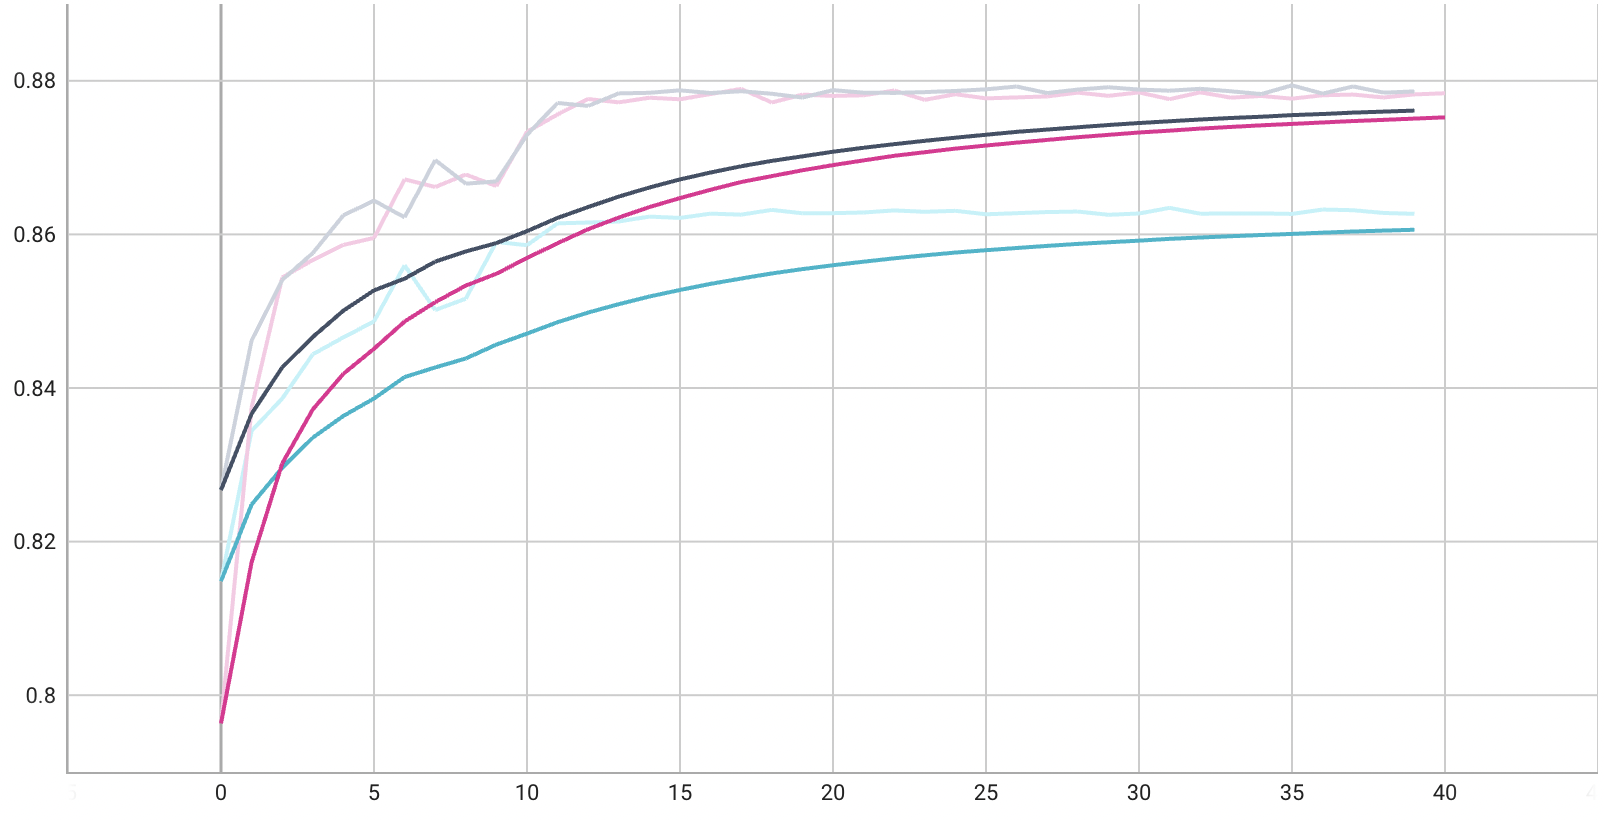
\includegraphics[width=9cm, height=5cm]{images/roads-losses/three-losses-iou.png}
    \caption{Progression of IoU Scores over 40 epochs for Focal Loss (Magenta), Dice Loss (Teal), and Cross Entropy Loss (Gray). U-Net network having a ResNet18 encoder pre-trained with ImageNet weights. The dataset doesn't have an imbalance. }
\end{figure}

\subsubsection{Network and Encoders} With an intent to observe the effect of the depth of network, we do a comparative analysis of ResNet18, ResNet34, and ResNet101. Additionally, we evaluate a U-Net++ network (using a ResNet34 encoder). All encoders are initialised with ImageNet weights. We train for a total of 40 epochs and employ Focal Loss as our loss function. The visualization results are shown in Fig 1. Fig 2,3,4 consist of graphs depicting the progession of metrics.

With an intent to observe the effect of the depth of network, we do a comparative analysis of ResNet18, ResNet34, and ResNet101. Additionally, we evaluate a U-Net++ network (using a ResNet34 encoder). All encoders are initialised with ImageNet weights. We train for a total of 40 epochs and employ Focal Loss as our loss function. The visualization results are shown in Fig 1. Fig 2,3,4 consist of graphs depicting the progession of metrics.

\begin{figure}[h]
    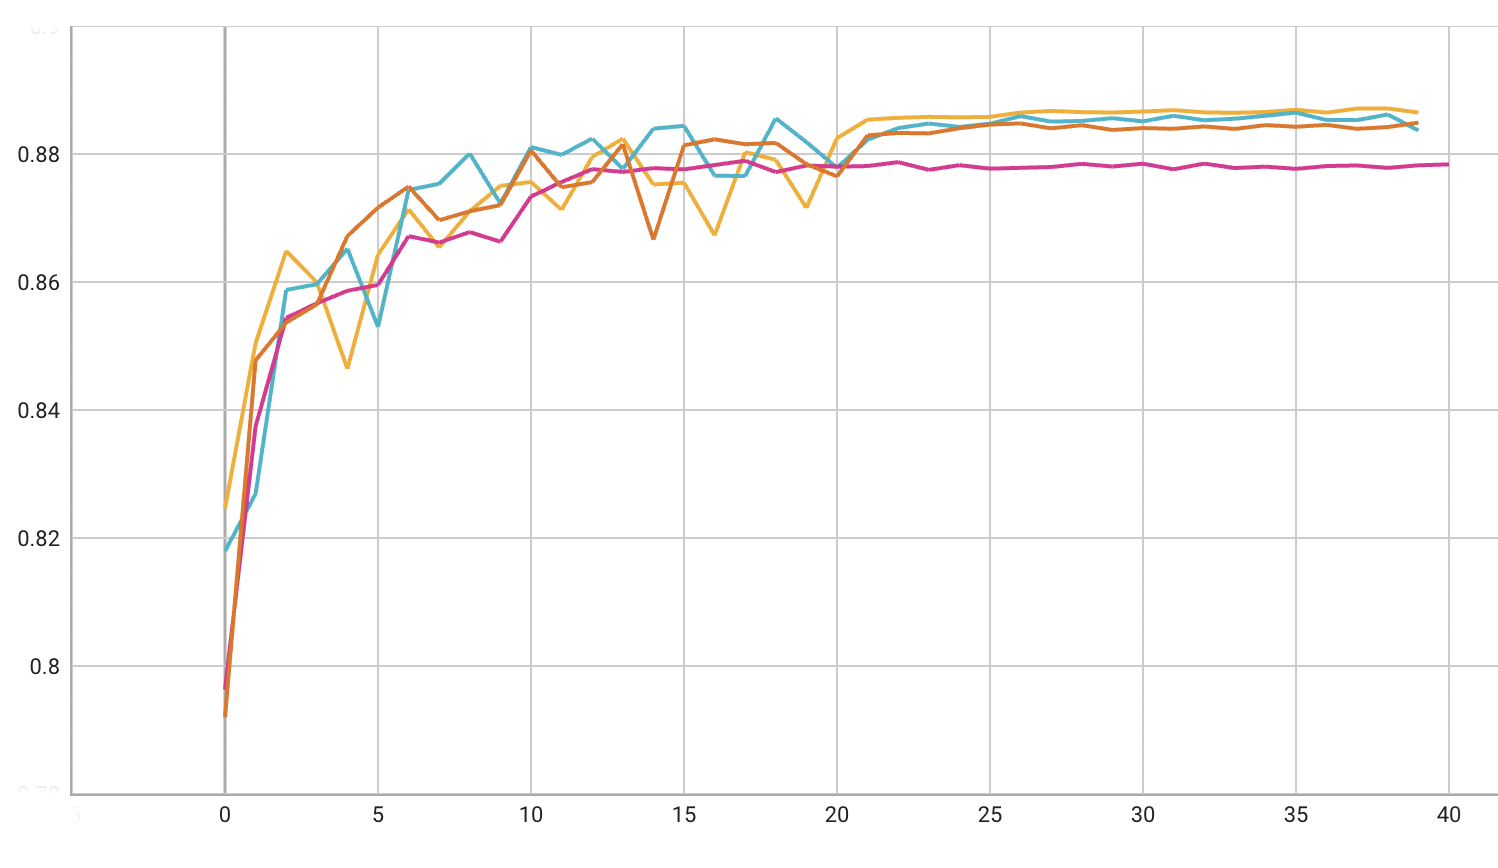
\includegraphics[width=9cm, height=5cm]{images/encoders/encoders_iou.png}
    \caption{Progression of IoU Scores over 40 epochs for U-Net ResNet18 (Pink), U-Net ResNet34 (Orange), U-Net ResNet101 (Blue), and U-Net++ ResNet34 (Yellow). Focal Loss is being employed and all encoders are initialized with pre-trained Image-Net weights.}
\end{figure}


% \begin{figure}[h]
%     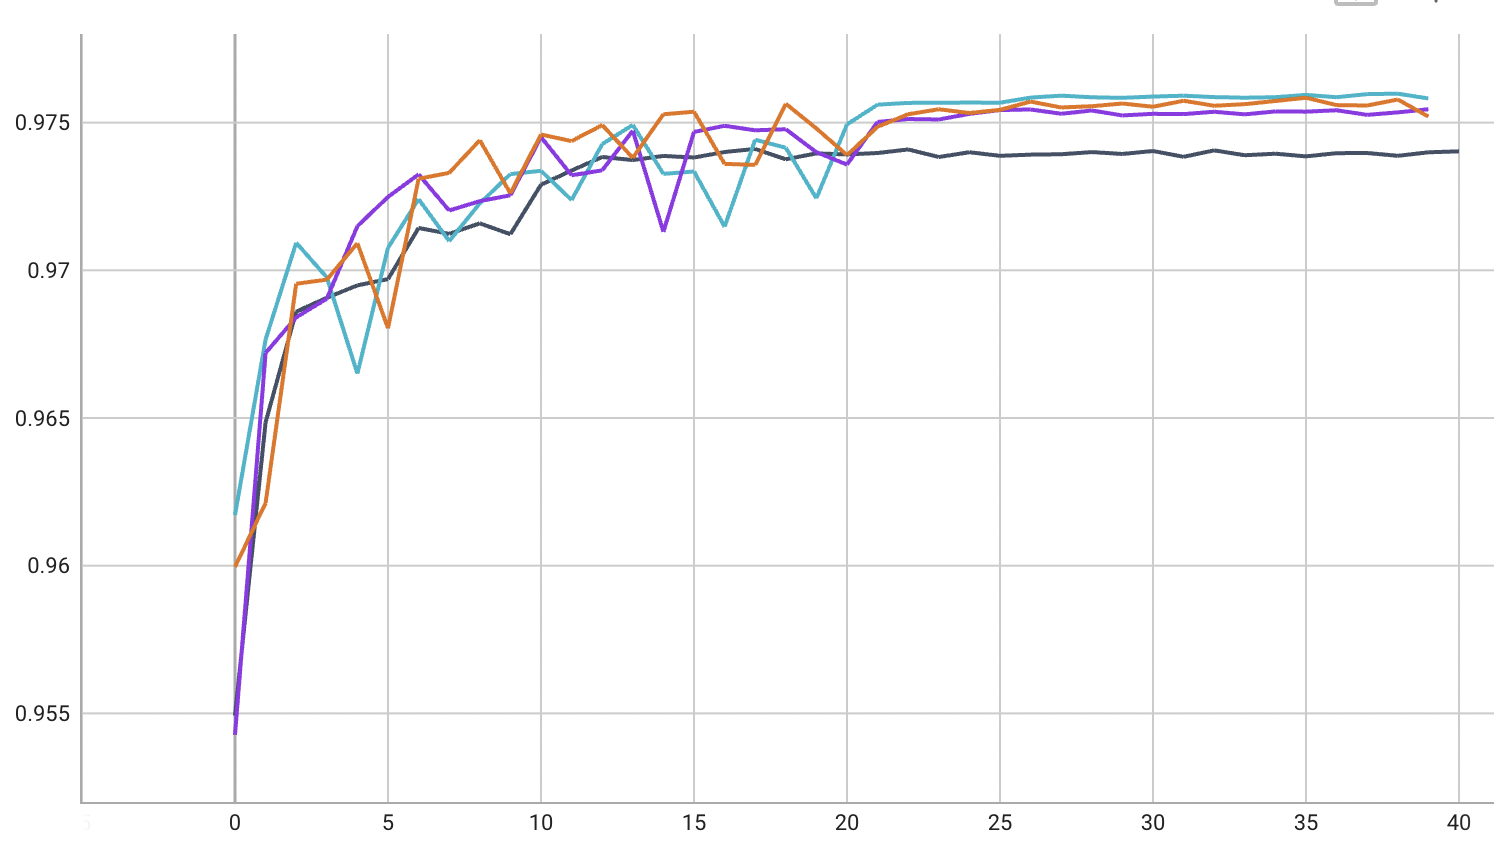
\includegraphics[width=9cm, height=5cm]{images/encoders/encoders_accuracy.png}
%     \caption{Progression of Pixel Accuracy over 40 epochs for U-Net ResNet18 (Dark Gray), U-Net ResNet34 (Purple), U-Net ResNet101 (Orange), and U-Net++ ResNet34 (Sky Blue). Focal Loss is being employed and all encoders are initialized with pre-trained Image-Net weights.}
% \end{figure}

\begin{figure}[h]
    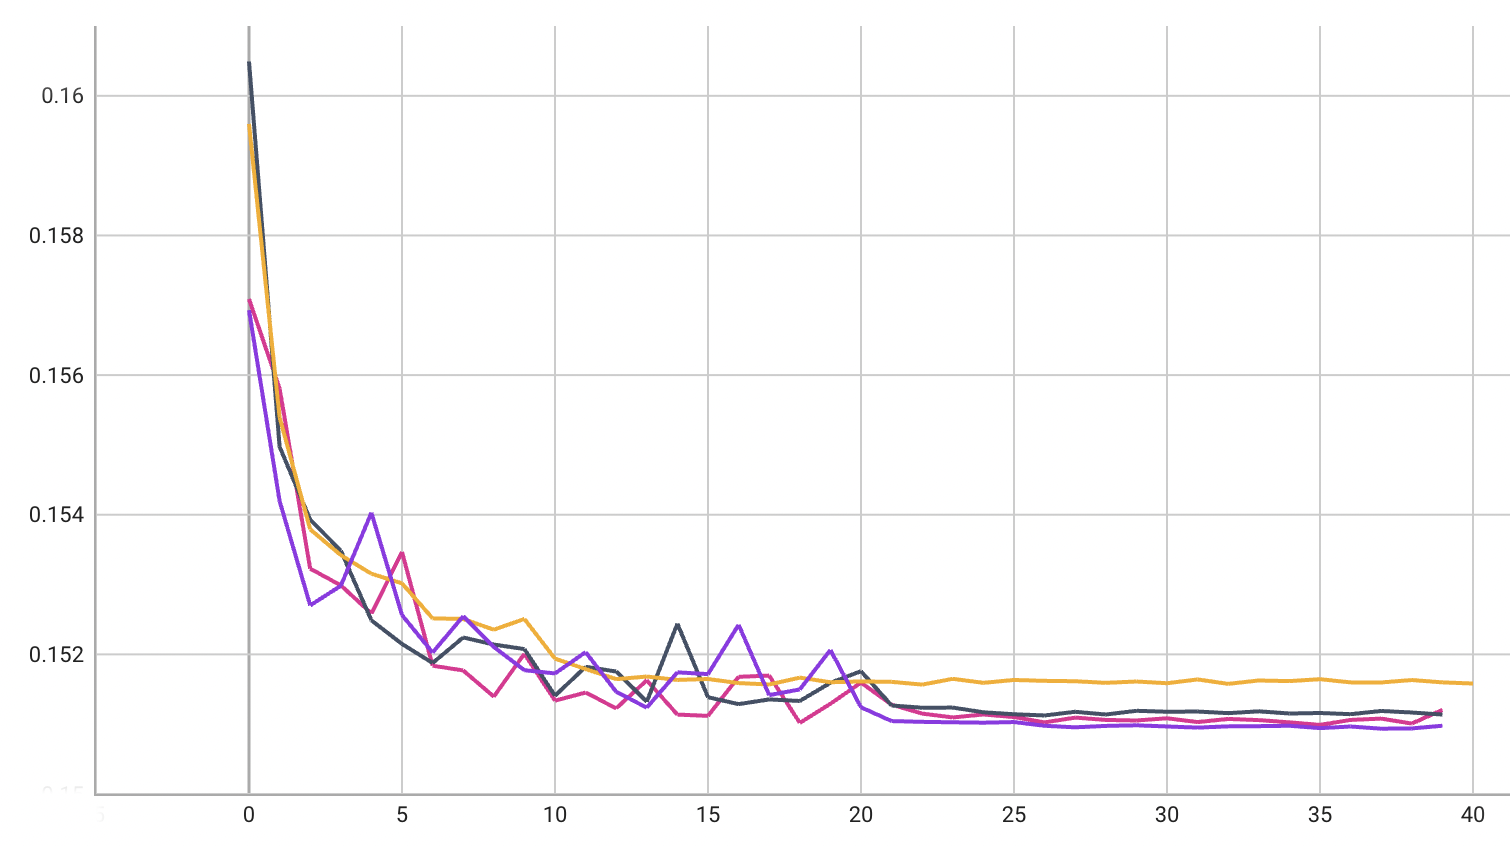
\includegraphics[width=9cm, height=5cm]{images/encoders/encoders_focalloss.png}
    \caption{Progression of Focal Loss values over 40 epochs for U-Net ResNet18 (Yellow), U-Net ResNet34 (Dark Gray), U-Net ResNet101 (Pink), and U-Net++ ResNet34 (Purple).}
\end{figure}

\begin{figure}[h]
    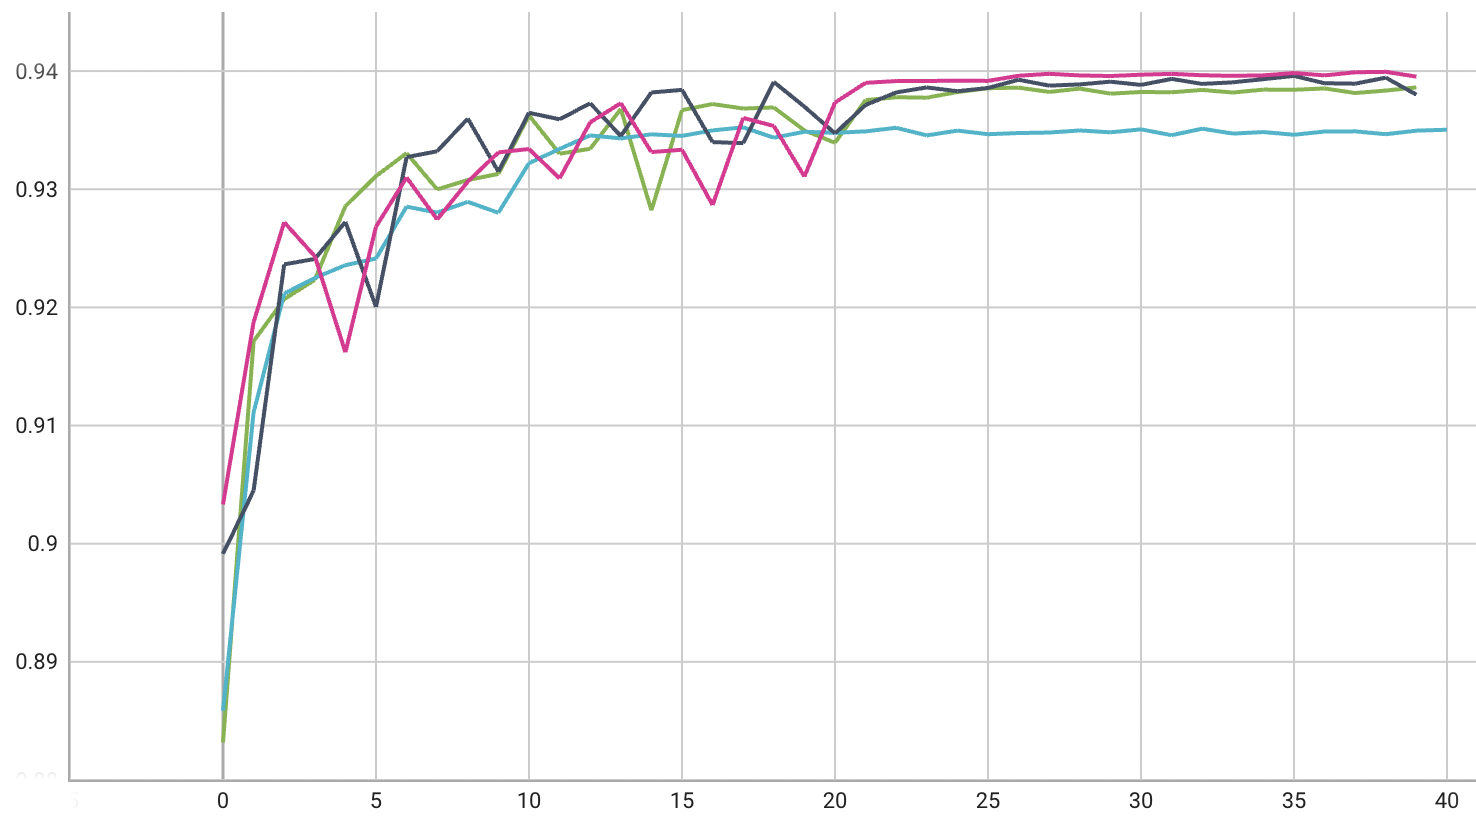
\includegraphics[width=9cm, height=5cm]{images/encoders/encoders_fscore.png}
    \caption{Progression of IoU Scores over 40 epochs for Focal Loss (Magenta), Dice Loss (Teal), and Cross Entropy Loss (Gray). U-Net network having a ResNet18 encoder pre-trained with ImageNet weights. The dataset doesn't have an imbalance. }
\end{figure}



\begin{figure*}
    \centering
    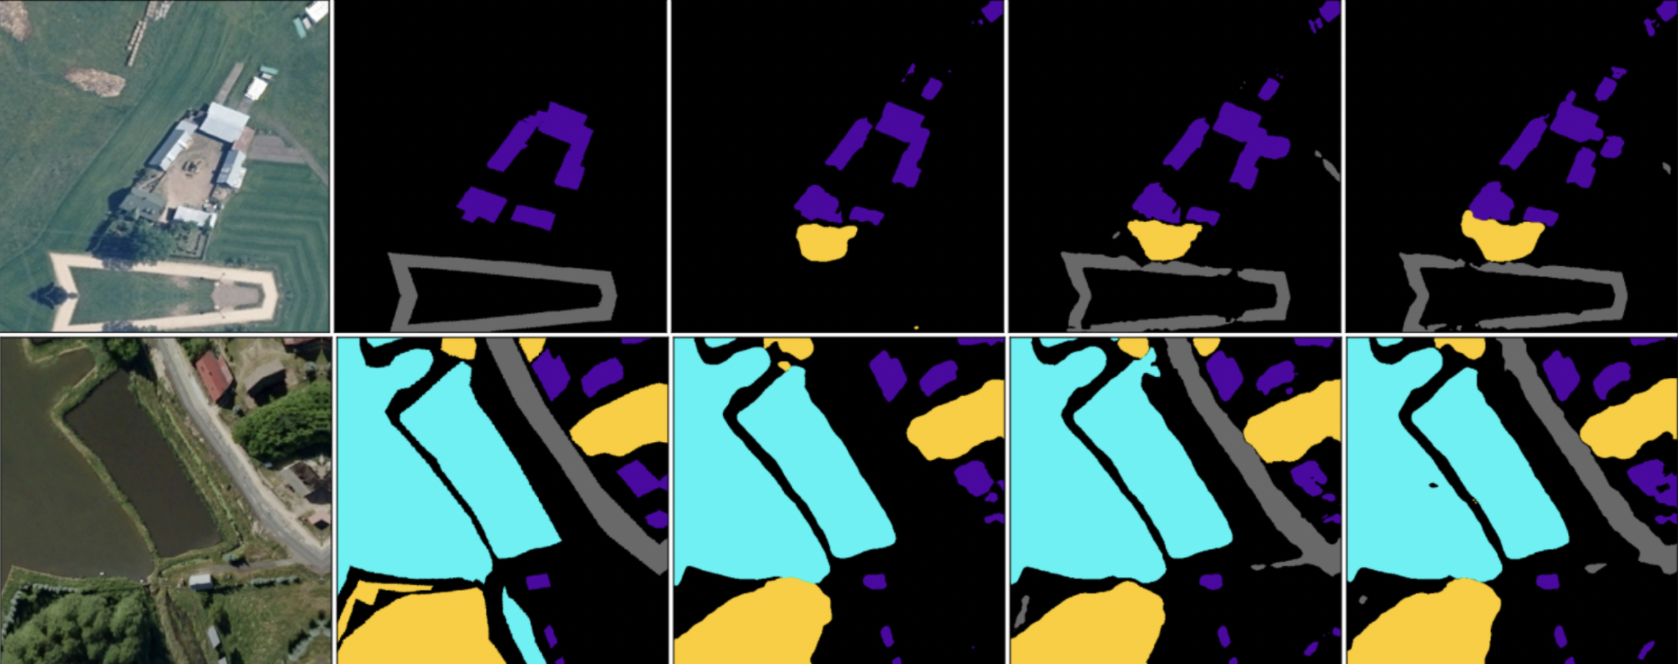
\includegraphics[width=\textwidth]{images/no-roads-losses/2-images.png}
    \caption{Prediction on a highly-imbalanced dataset with a U-Net network on a ResNet18 encoder. The first column contains the actual images, the second column represents the target mask, the third, fourth, and fifth columns represent the predicted mask with Dice, Focal, and Cross Entropy Loss respectively. Dice Loss(third columns) fails to detect the minority class (roads) in a lot of samples}
\end{figure*}

\begin{figure*}[h]
    \centering
    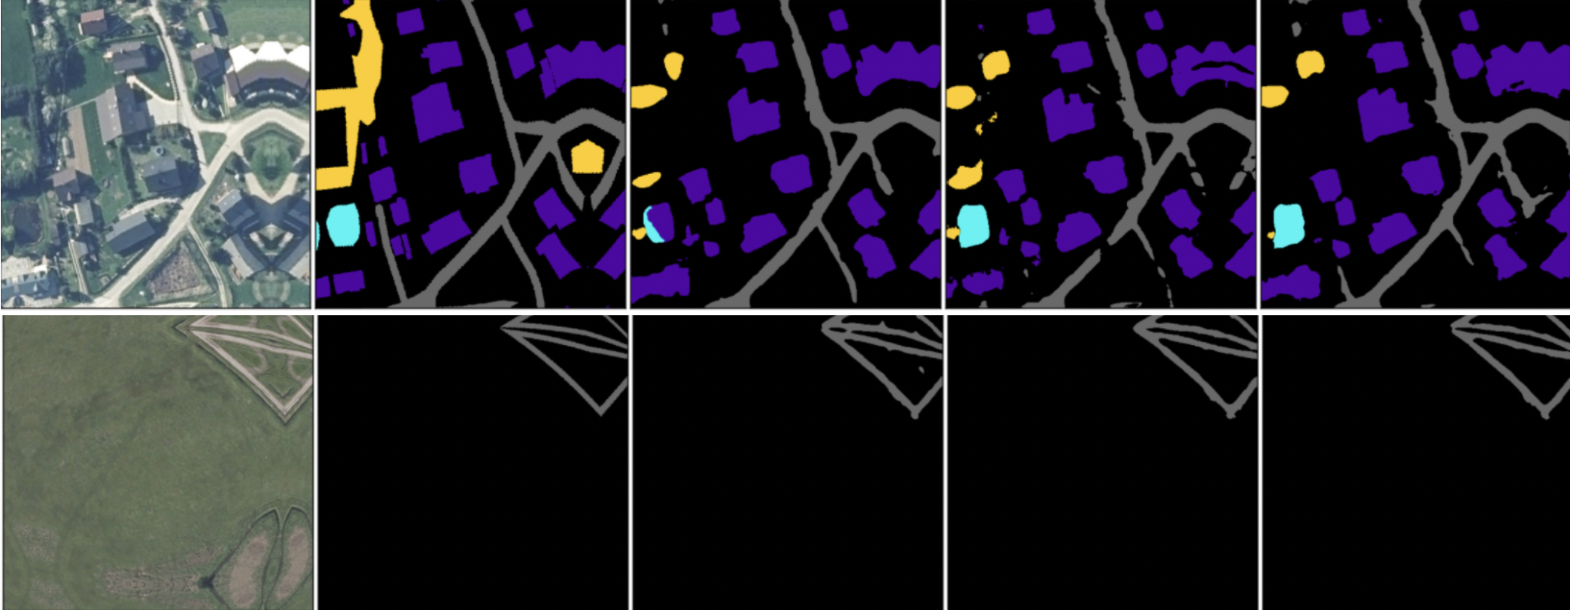
\includegraphics[width=\textwidth]{images/roads-losses/with-roads.png}
    \caption{Prediction on a more balanced dataset with a U-Net network on a ResNet18 encoder. The first column contains the actual images, the second column represents the target mask, the third, fourth, and fitth columns represent the Predicted Mask with Dice, Focal, and Cross Entropy Loss respectively}
\end{figure*}


% ============================
\section{Results}
% ============================
\begin{enumerate}
    \item Focal Loss performs the best in scenarios of data imbalance. On the other hand, IoU values remain comparable between the three loss functions when the dataset is slightly balanced.
    \item ResNet50 performs best vs 18 and 34
    \item U-Net++ provides a better.
\end{enumerate}
% ============================
\section{Conclusion}
% ============================



\bibliographystyle{ACM-Reference-Format}
\bibliography{bibliography}

\end{document}